\documentclass{article}

\usepackage{booktabs}
\usepackage{tabularx}
\usepackage{hyperref}
\usepackage{tabularray}
\usepackage{float}
\usepackage{graphicx}
\UseTblrLibrary{booktabs}

\hypersetup{
    colorlinks=true,       % false: boxed links; true: colored links
    linkcolor=red,          % color of internal links (change box color with linkbordercolor)
    citecolor=green,        % color of links to bibliography
    filecolor=magenta,      % color of file links
    urlcolor=cyan           % color of external links
}

\title{PronouncedFish Wireframe Report\\\progname}

\author{\authname}

\date{}

\input{../../Comments.text}
\input{../../Common.text}

\begin{document}

\maketitle
\thispagestyle{empty}

~\newpage

\pagenumbering{roman}

\begin{table}[hp]
\caption{Revision History} \label{TblRevisionHistory}
\begin{tabularx}{\textwidth}{llX}
\toprule
\textbf{Date} & \textbf{Developer(s)} & \textbf{Change}\\
\midrule
18/11/2026 & Lily Porter & First submission\\
 & & \\
\bottomrule
\end{tabularx}
\end{table}

~\newpage

\tableofcontents

~\newpage

\pagenumbering{roman}

\section{Purpose \& Scope}

This report outlines the PronouncedFish initial user interface wireframes and mock-ups that were presented to the project supervisors, and the resulting insights gathered during review. The purpose of the review was for the supervisors to comment on the information displayed, user interaction patterns, and visual design before a final user interface is finalized.

The wireframes presented in this report are initial stage design representations rather than a complete specification of the system's final behaviour, details that will be finalized based off supervisor feedback and further work on the project. The wireframes were designed to illustrate the key features of the system's user interface:
\begin{enumerate}
    \item The clinician (SLP) facing dashboard, used to review patient progress, data, and prepare session activities.
    \item The child-facing experience, used by the SLP during a speech practice session with a patient.
\end{enumerate}

\section{Wireframe Overview \& Review Context}

The child-facing interface takes on an ocean/coral reef theme, intended to fit the theme of project name, PronouncedFish. It features simple picture cues, engaging character icons, and simple controls that make the session feel approachable and fun for the patient. The SLP-facing interface is more information-dense, presenting important information to the SLP such as session schedules, session data, progress visualizations, and activity setup.

This wireframe review was conducted with the project supervisors, Dr.\ Lyn Turkstra and Dr.\ Daniel Pape. Dr.\ Turkstra is a licensed speech-language pathologist and Assistant Dean and Professor of Speech-Language Pathology in the School of Rehabilitation Sciences. Dr.\ Pape is an Associate Professor in the Department of Linguistics and Languages at McMaster University.

\section{Wireframe Walkthrough}

\subsection{SLP-Facing Dashboard and Interface}

The following mock-ups represent the SLP dashboard and workflow, when there is not currently an ongoing patient session. They include features for an SLP such as viewing a list of their upcoming appointments, data analysis of sessions, and practice plans for their patients.

\subsubsection{Wireframe 1}

This represents the high-level caseload and session overview that an SLP requires. It presents patient cases requiring review, active caseloads, session schedules during a selected week, and other key details an SLP may want to view on the overview page.

\begin{figure}[h!]
\begin{center}
\rotatebox{0}
{
  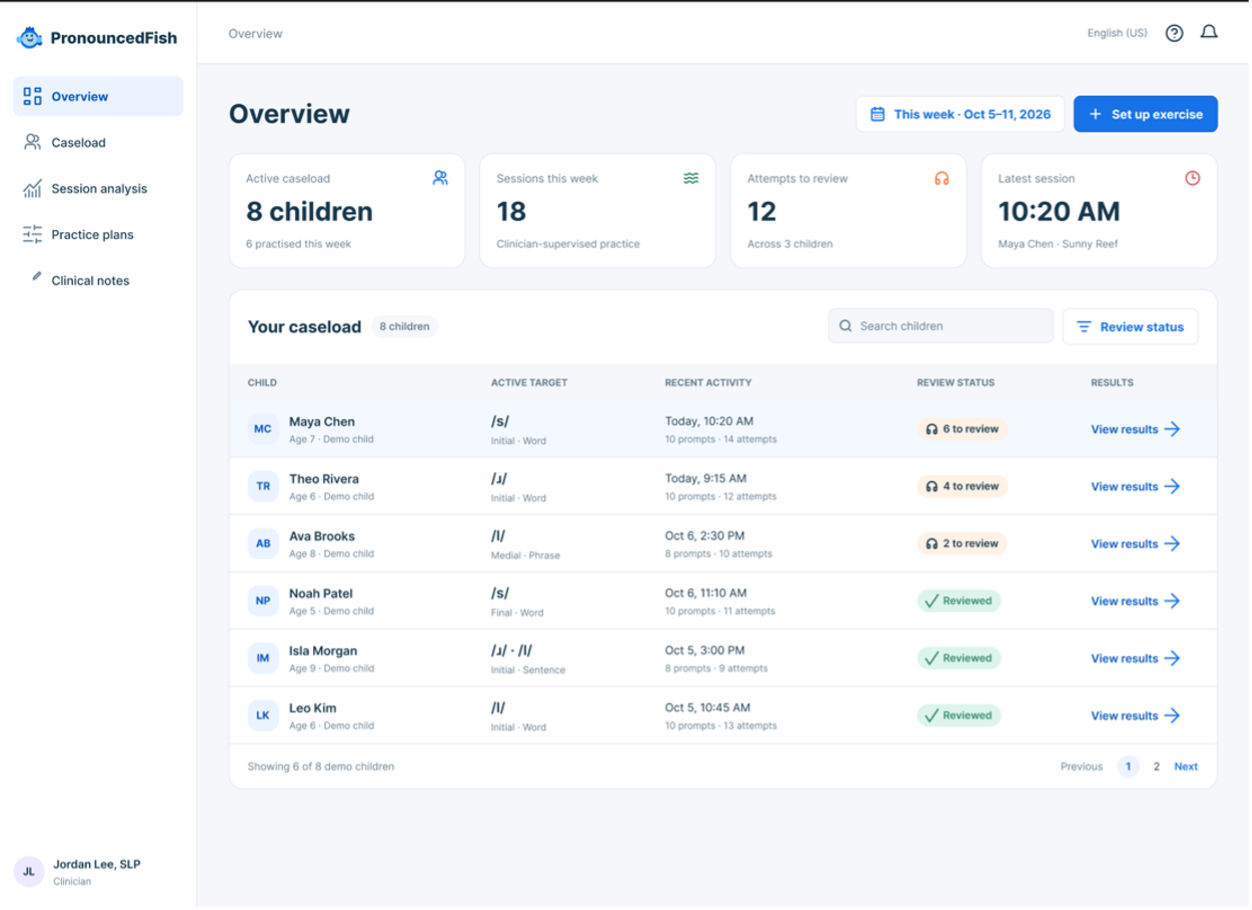
\includegraphics[width=0.5\textwidth]{W1.png}
}
\caption{\label{<Label>} Wireframe 1}
\end{center}
\end{figure}

\subsubsection{Wireframe 2}

This represents what an SLP may want to view for session analysis. It shows data visualizations for phoneme targets, accuracy estimates and trends, session attempts, and playback controls.

\begin{figure}[h!]
\begin{center}
\rotatebox{0}
{
  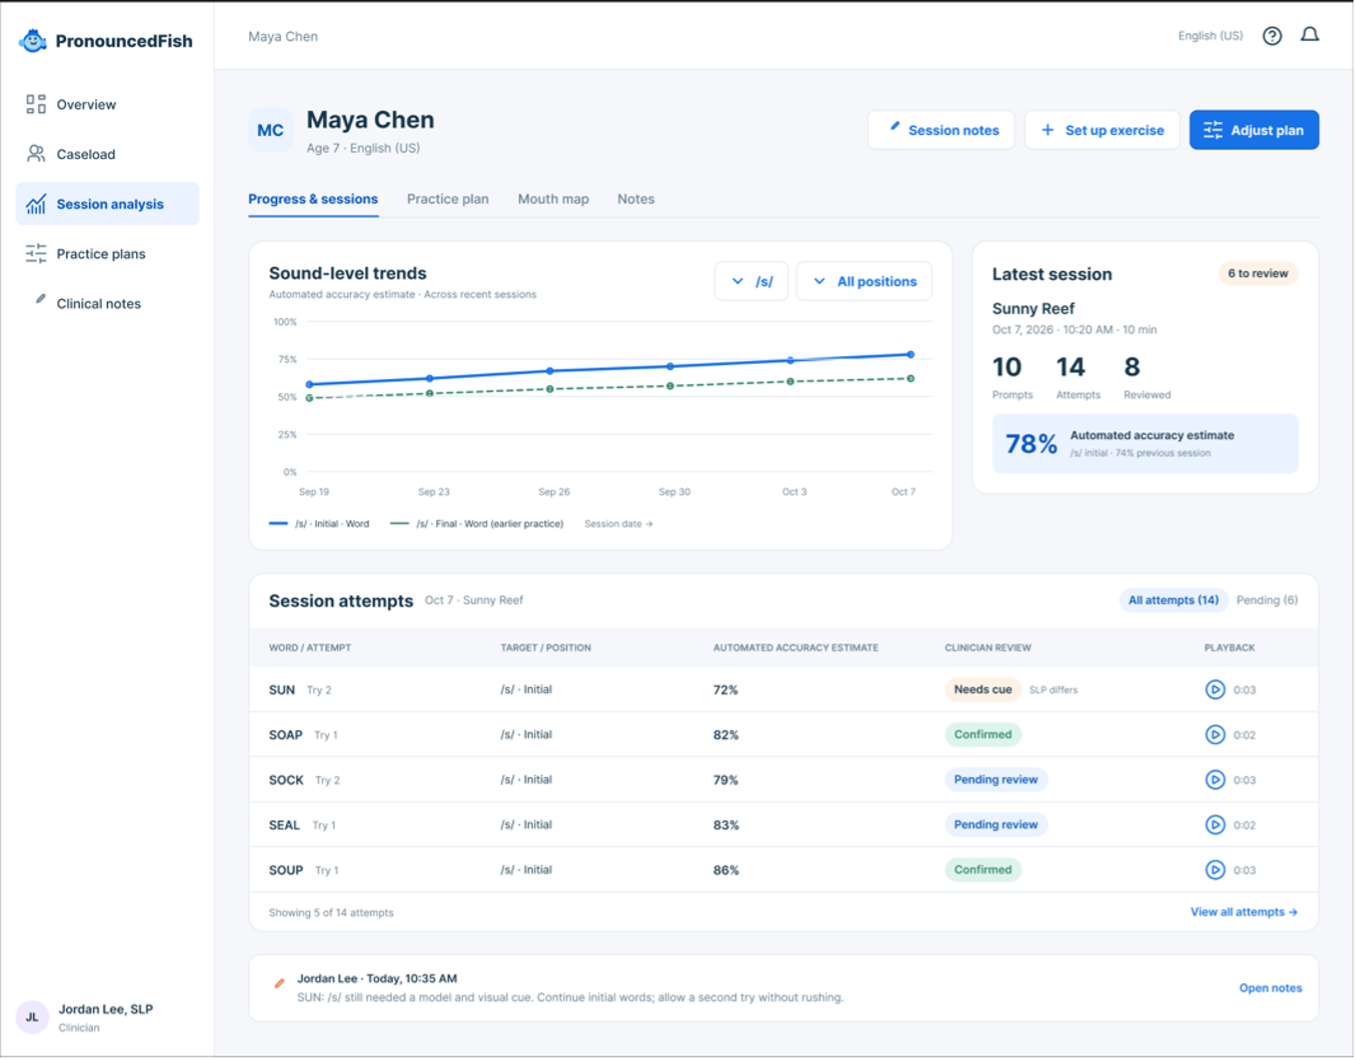
\includegraphics[width=0.5\textwidth]{W2.png}
}
\caption{\label{<Label>} Wireframe 2}
\end{center}
\end{figure}

\subsubsection{Wireframe 3}

This represents another potential view option for session analysis. The represented visualization illustrates a mouth-placement map. This visualization would show the SLP where a selected sound in a session was produced in the mouth and include its place of articulation, and information on voicing. This wireframe was created upon previous supervisor feedback and insight that a data visualization of this manner would be useful.

\begin{figure}[h!]
\begin{center}
\rotatebox{0}
{
  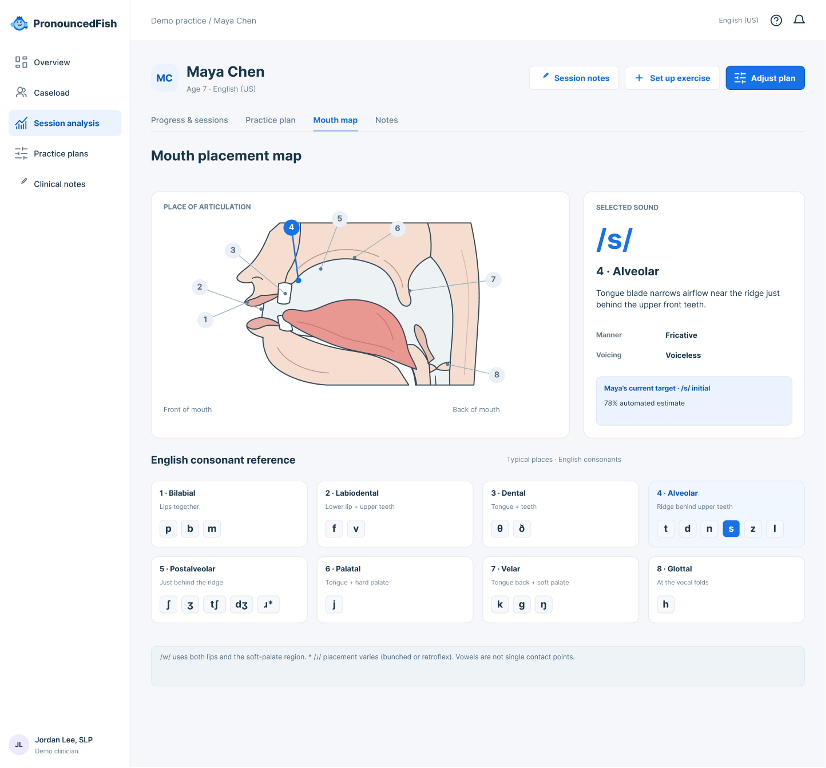
\includegraphics[width=0.5\textwidth]{W3.png}
}
\caption{\label{<Label>} Wireframe 3}
\end{center}
\end{figure}

\subsubsection{Wireframe 4}

This represents a feature which would allow an SLP to add and adjust practice plans for their patients. It includes options to configure a target sound/phoneme, word position, pacing, and repetition.

\begin{figure}[h!]
\begin{center}
\rotatebox{0}
{
  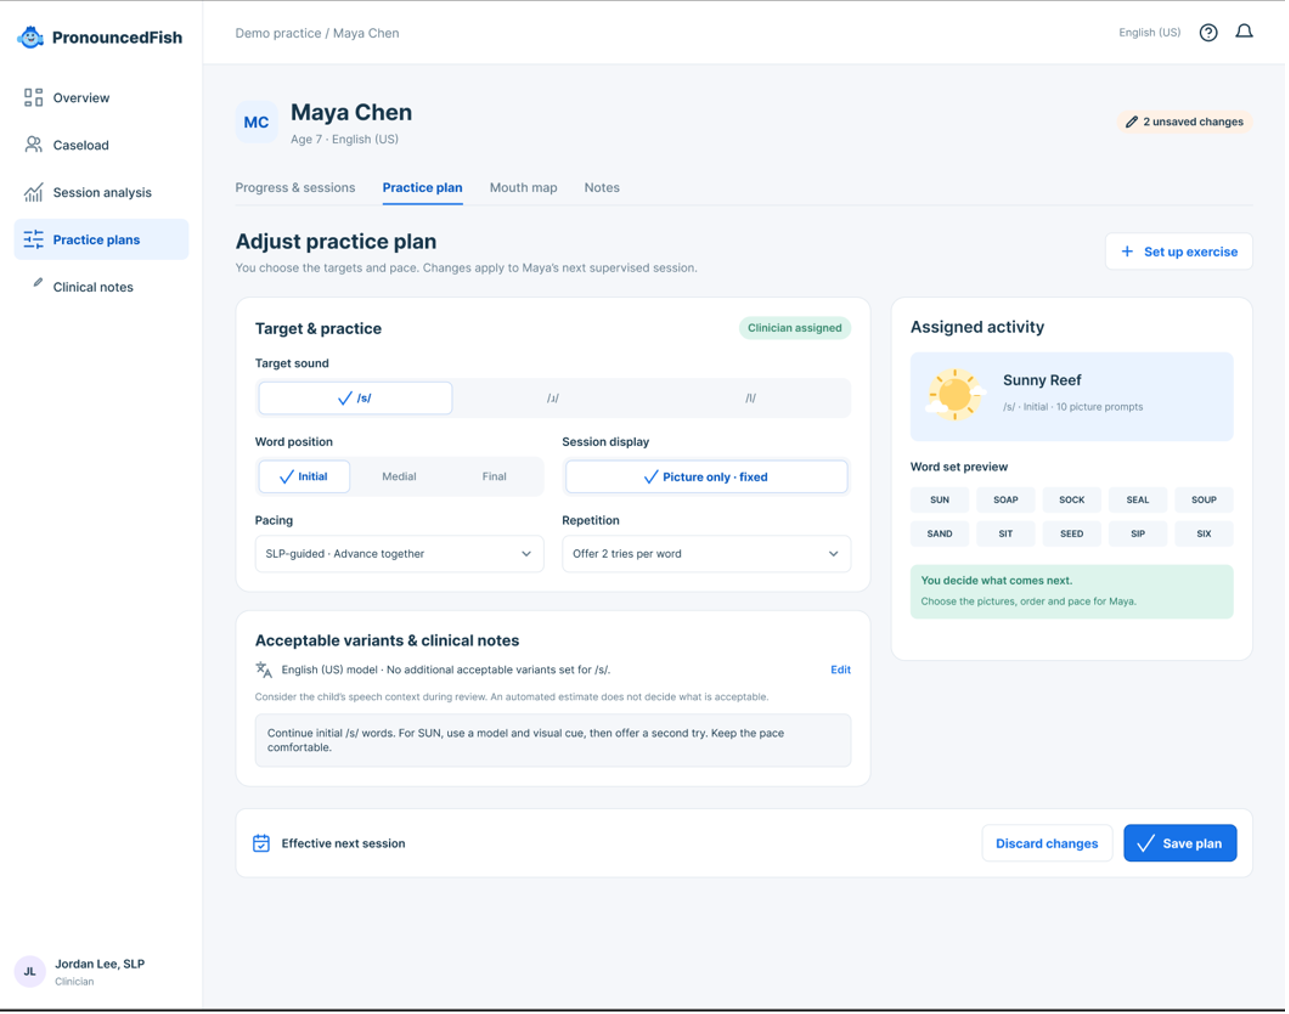
\includegraphics[width=0.5\textwidth]{W4.png}
}
\caption{\label{<Label>} Wireframe 4}
\end{center}
\end{figure}

\subsubsection{Wireframe 5}

This represents another potential design for an SLP's practice plans. It shows a feature which would allow an SLP to select a target word and picture prompt and preview what a patient would see during a session.

\begin{figure}[h!]
\begin{center}
\rotatebox{0}
{
  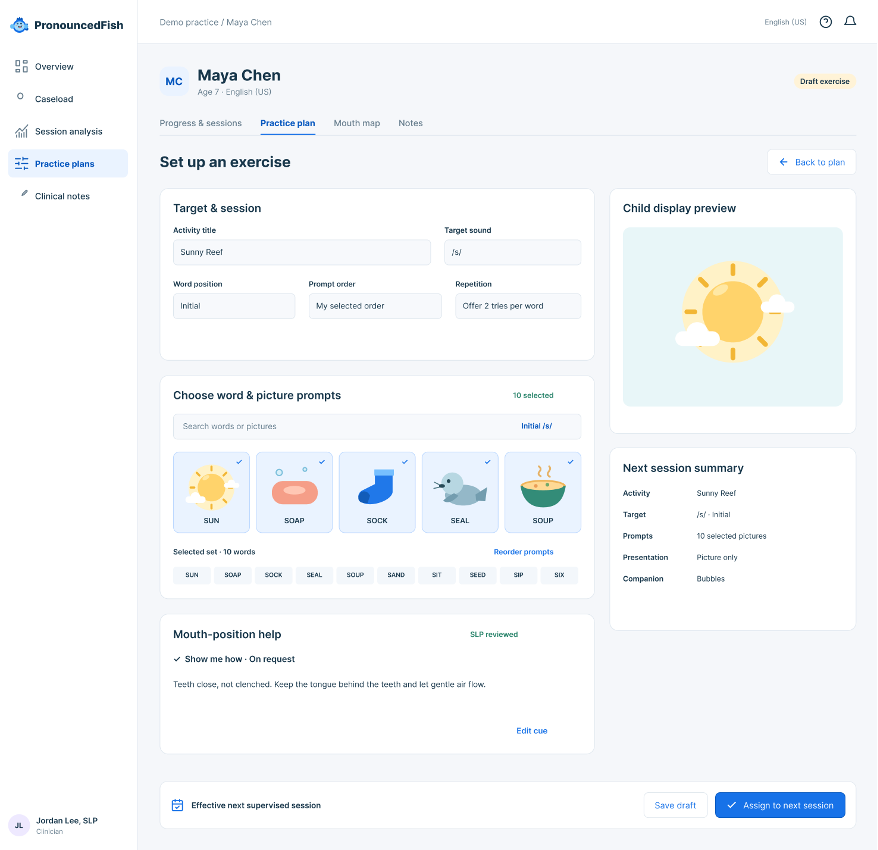
\includegraphics[width=0.5\textwidth]{W5.png}
}
\caption{\label{<Label>} Wireframe 5}
\end{center}
\end{figure}

\subsection{Patient-Facing (In-Session) Interface}

The following mock-ups represent what the screen would show when a session has been started. It is designed to be accessible and engaging to a child patient as the SLP goes through the practice items with them.

\subsubsection{Wireframe 6}

This represents what would be shown once a session is started. It is a start screen that establishes the theme before the practice begins.

\begin{figure}[h!]
\begin{center}
\rotatebox{0}
{
  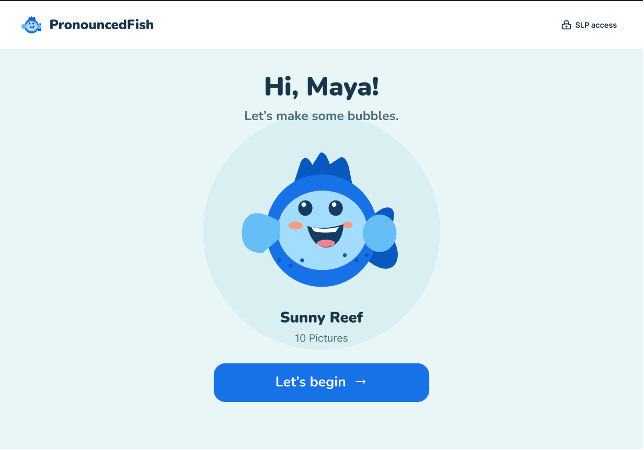
\includegraphics[width=0.5\textwidth]{W6.png}
}
\caption{\label{<Label>} Wireframe 6}
\end{center}
\end{figure}

\subsubsection{Wireframe 7}

This represents how a practice item would be presented during a session. ``Tap to Speak'' would be tapped when the practice is attempted.

\begin{figure}[h!]
\begin{center}
\rotatebox{0}
{
  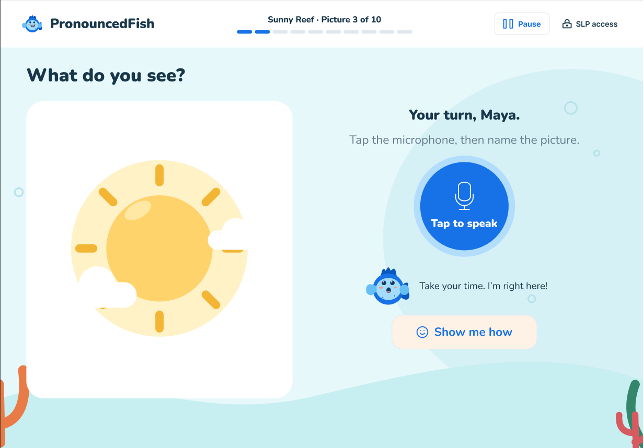
\includegraphics[width=0.5\textwidth]{W7.png}
}
\caption{\label{<Label>} Wireframe 7}
\end{center}
\end{figure}

\subsubsection{Wireframe 8}

This represents the results that would be shown after a practice item is attempted. It is meant to be supportive without making an unsuccessful attempt feel discouraging to a patient.

\begin{figure}[h!]
\begin{center}
\rotatebox{0}
{
  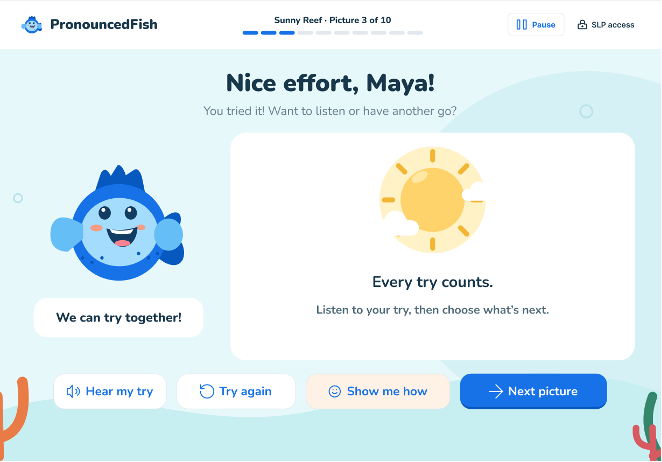
\includegraphics[width=0.5\textwidth]{W8.png}
}
\caption{\label{<Label>} Wireframe 8}
\end{center}
\end{figure}

\subsubsection{Wireframe 9}

This represents what the interface shows when a session has been completed. It summarizes the activities that were performed.

\begin{figure}[h!]
\begin{center}
\rotatebox{0}
{
  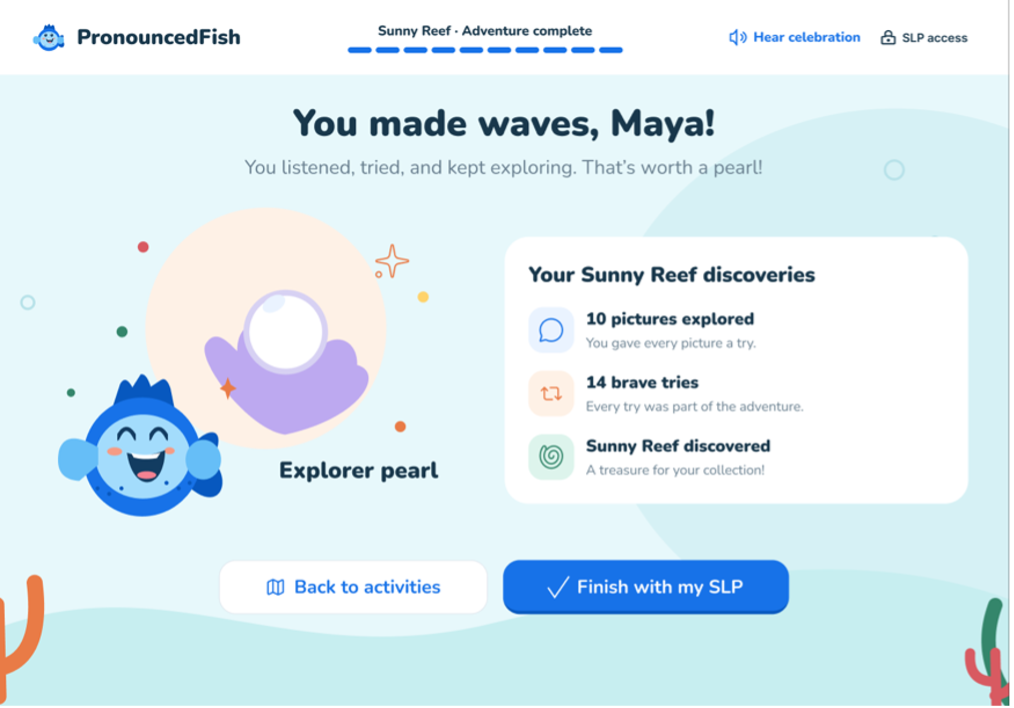
\includegraphics[width=0.5\textwidth]{W9.png}
}
\caption{\label{<Label>} Wireframe 9}
\end{center}
\end{figure}

\subsubsection{Wireframe 10}

This represents a practice activity with visual guidance on how a patient should attempt to make a sound.

\begin{figure}[h!]
\begin{center}
\rotatebox{0}
{
  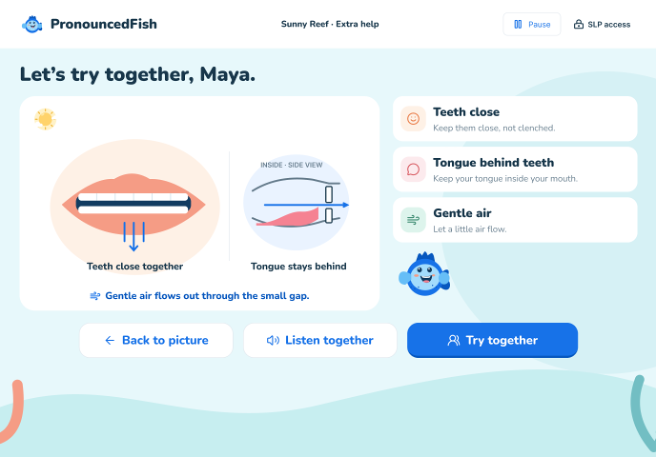
\includegraphics[width=0.5\textwidth]{W10.png}
}
\caption{\label{<Label>} Wireframe 10}
\end{center}
\end{figure}

\section{Supervisor Feedback \& Insights}

Feedback from supervisors related to how the interface should distinguish between patient assessment and treatment sessions, availability and presentation of audio recordings, configurable practice sessions, and balancing a child-friendly session presentation with clinically meaningful information.

\subsection{Keeping Assessment and Therapy Session Content Distinct}

One key insight from our supervisors was to refer to the Goldman-Fristoe test for SLP patient assessment. The Goldman-Fristoe test is a standardized assessment used by speech-language pathologists (SLPs) to measure how well a person produces consonant sounds and identifies speech sound disorders. This test is typically administered at the beginning of a therapy case (in the first session) and again at the end of therapy treatment (the final session), to have a standardized measurement of speech challenges and overall improvement from therapy. SLPs use the results of this test to guide their treatment plan for a patient's speech therapy.

The feedback provided clarified that the system should contain functionality for administering this formal test and that the test sets should not carry over into the therapy practice sets.

The supervisors also raised the possibility of targeting sounds in sentences rather than only looking at individual words.

\subsection{Audio Recording Playback and Availability}

Having an option for playback of a speech attempt was identified by the supervisors as useful for reviewing a patient's progress. The audio files must be long enough to support scoring.

Feedback also discussed how long audio files should be stored/retained and available on the dashboard. It was clarified that speech therapy blocks are typically around 10-weeks. The suggestion was to allow for the storage and interface availability of audio recordings until a patient's therapy block is complete and deleted afterwards.

\subsection{Data and Results Visualizations}

The supervisor feedback noted that data visualizations for word sound positions (initial, medial, final) would be very helpful to include for session analysis. There are also categories specified in the Goldman-Fristoe test that would be useful to incorporate into the interface visualizations.

The supervisors also suggested that SLPs should be able to select which errors to target when looking at session data visualizations.

The supervisors also emphasized that a review process for the speech results would be helpful. In the interface correct pronunciations could be marked with a checkmark, while incorrect pronunciations could be marked with an x. The interface should make it clear which results are automated results and which have been reviewed or confirmed by the SLP.

It was also noted that the accuracy of the visual aids in the wireframes could be improved. The mouth and face visualizations should be anatomically correct and easily decipherable by the user. Any provided image cues for practice items should also be clear and easy to identify.

\section{Conclusion}

The wireframe review helped clarify that PronouncedFish must support two connected but different experiences: an efficient workflow for the SLP, and an encouraging and interactive in-session interface. The most important insights gained related to the separation of the patient assessment and patient therapy activities, and the specification of what data visualizations would be most helpful to an SLP.

\newpage{}

\section{Appendix --- Generative AI Use Disclosure}

\subsection{AI Tools Used}

ChatGPT-6 was used.

\subsection{How and Where Used}

AI was used for converting a written word doc version of the report to LaTeX code. It was also used to brainstorm the outline/subsections to be included in the report. 

\subsection{Verification of AI-Generated Content}

The generated LaTeX file was compared against the written Word document to verify that content remained the same and all written wording was preserved.

\end{document}